% ============================================================
% VECTORS: THE LANGUAGE OF DATA
% Beamer + Manim Animated Presentation
% Author: Dr Milan Joshi
% Theme: Blueprint Noir — cinematic, minimal, architectural
% ============================================================

\documentclass[aspectratio=169, 10pt]{beamer}

% ============================================================
% PACKAGES
% ============================================================
\usepackage{animate}        % Frame-by-frame animation in PDF
\usepackage{graphicx}       % Image inclusion
\usepackage{amsmath}        % Math typesetting
\usepackage{amssymb}        % Math symbols
\usepackage{xcolor}         % Color definitions
\usepackage{tikz}           % Drawing
\usetikzlibrary{calc,positioning,arrows.meta,decorations.pathreplacing}
\usepackage{booktabs}       % Better tables
\usepackage{fontenc}[T1]
\usepackage{textcomp}
\usepackage{bm}             % Bold math
\usepackage{multicol}       % Multi-column layouts
\usepackage{mathtools}      % Extra math tools

% ============================================================
% COLOR PALETTE — "Blueprint Noir"
% ============================================================
\definecolor{bgdark}{HTML}{0B0B1A}
\definecolor{gridcolor}{HTML}{1A1A3A}
\definecolor{textwhite}{HTML}{EEEEFF}
\definecolor{vectora}{HTML}{4FC3F7}      % Electric Blue
\definecolor{vectorb}{HTML}{FF8A65}      % Warm Orange
\definecolor{resultant}{HTML}{66BB6A}    % Vibrant Green
\definecolor{projection}{HTML}{AB47BC}   % Soft Purple
\definecolor{labelgray}{HTML}{B0BEC5}    % Neutral Gray
\definecolor{accent}{HTML}{FFD54F}       % Gold
\definecolor{codebg}{HTML}{111128}       % Code background
\definecolor{cardbg}{HTML}{12122A}       % Card background

% ============================================================
% BEAMER THEME CONFIGURATION — Dark Cinematic
% ============================================================
\usetheme{default}
\usecolortheme{default}

% Background
\setbeamercolor{background canvas}{bg=bgdark}

% Title
\setbeamercolor{frametitle}{fg=textwhite}
\setbeamerfont{frametitle}{size=\Large, series=\bfseries}

% Text
\setbeamercolor{normal text}{fg=textwhite}
\setbeamercolor{itemize item}{fg=vectora}
\setbeamercolor{itemize subitem}{fg=accent}
\setbeamercolor{enumerate item}{fg=vectora}

% Bullets
\setbeamertemplate{itemize item}{\small\raise1pt\hbox{\textcolor{vectora}{$\blacktriangleright$}}}
\setbeamertemplate{itemize subitem}{\small\raise1pt\hbox{\textcolor{accent}{$\circ$}}}

% Remove navigation symbols
\setbeamertemplate{navigation symbols}{}

% Footer with slide number
\setbeamertemplate{footline}{%
  \hfill%
  \textcolor{labelgray}{\footnotesize\insertframenumber\,/\,\inserttotalframenumber}%
  \hspace{6pt}\vspace{4pt}%
}

% Block styling
\setbeamercolor{block title}{fg=bgdark, bg=vectora}
\setbeamercolor{block body}{fg=textwhite, bg=codebg}
\setbeamercolor{block title alerted}{fg=bgdark, bg=vectorb}
\setbeamercolor{block body alerted}{fg=textwhite, bg=codebg}
\setbeamercolor{block title example}{fg=bgdark, bg=resultant}
\setbeamercolor{block body example}{fg=textwhite, bg=codebg}

% ============================================================
% CUSTOM COMMANDS
% ============================================================
\newcommand{\vecb}[1]{\mathbf{#1}}
\newcommand{\norm}[1]{\left\| #1 \right\|}
\newcommand{\modulemark}[1]{%
  \textcolor{accent}{\scriptsize\textbf{MODULE #1}}%
}
\newcommand{\concepttag}[1]{%
  \textcolor{labelgray}{\scriptsize #1}%
}
\newcommand{\excard}[3]{%
  \colorbox{cardbg}{\parbox{0.43\textwidth}{%
    \vspace{4pt}%
    \textcolor{#1}{\textbf{\small #2}}\\[2pt]%
    {\scriptsize\textcolor{textwhite}{#3}}%
    \vspace{4pt}%
  }}%
}
\newcommand{\minicard}[3]{%
  \colorbox{cardbg}{\parbox{0.28\textwidth}{%
    \vspace{3pt}%
    \textcolor{#1}{\textbf{\scriptsize #2}}\\[2pt]%
    {\tiny\textcolor{textwhite}{#3}}%
    \vspace{3pt}%
  }}%
}

% ============================================================
% TITLE PAGE INFO
% ============================================================
\title{\textcolor{vectora}{\Huge Vectors}}
\subtitle{\textcolor{accent}{The Language of Data}}
\author{\textcolor{textwhite}{Dr Milan Joshi}}
\date{}


% ============================================================
% BEGIN DOCUMENT
% ============================================================
\begin{document}

% ============================================================
% SLIDE 1: Title Slide
% ============================================================
\begin{frame}[plain]
  \vfill
  \begin{center}
    
\begin{tikzpicture}[remember picture, overlay]
      \foreach \x in {-8,-7,...,8} {
        \draw[gridcolor, line width=0.2pt, opacity=0.3] (\x,-5) -- (\x,5);
      }
      \foreach \y in {-5,-4,...,5} {
        \draw[gridcolor, line width=0.2pt, opacity=0.3] (-8,\y) -- (8,\y);
      }
      \draw[-{Stealth[length=6pt]}, vectora, line width=1.5pt, opacity=0.15]
        (-4,-2) -- (3,2.5);
      \draw[-{Stealth[length=5pt]}, vectorb, line width=1.2pt, opacity=0.12]
        (-2,-3) -- (4,1);
    \end{tikzpicture}
    \vspace{1.5cm}
    {\Huge\bfseries\textcolor{vectora}{Vectors}\par}
    \vspace{0.3cm}
    {\Large\textcolor{accent}{The Language of Data}\par}
    \vspace{0.15cm}
    {\small\textcolor{labelgray}{A Data Structure Perspective}\par}
    \vspace{1.0cm}
    {\normalsize\textcolor{textwhite}{Dr Milan Joshi}\par}
    \vfill
    {\tiny\textcolor{labelgray}{Interactive PDF \textemdash\ Best viewed in Adobe Acrobat Reader}\par}
    \vspace{0.3cm}
  \end{center}
\end{frame}


% ============================================================
% MODULE 1: What is a Vector?
% ============================================================

% SLIDE 2: Three Perspectives
\begin{frame}{What is a Vector? \textemdash\ Three Perspectives}
  \modulemark{1} \hfill \concepttag{Intuition First}
  \vspace{0.3cm}

  \begin{columns}[T]
    \begin{column}{0.30\textwidth}
      \begin{center}
        \textcolor{vectora}{\textbf{\large Physicist}}\\[6pt]
        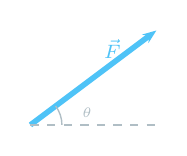
\begin{tikzpicture}[scale=0.8]
          \draw[-{Stealth[length=5pt]}, vectora, line width=2pt]
            (0,0) -- (2, 1.5);
          \node[vectora, font=\scriptsize] at (1.3, 1.2) {$\vec{F}$};
          \draw[labelgray, dashed, line width=0.5pt] (0,0) -- (2,0);
          \draw[labelgray, line width=0.5pt] (0.5,0) arc[start angle=0, end angle=37, radius=0.5];
          \node[labelgray, font=\tiny] at (0.9, 0.2) {$\theta$};
        \end{tikzpicture}
      \end{center}
      \vspace{0.15cm}
      {\scriptsize An arrow with \textcolor{vectora}{magnitude} and \textcolor{vectora}{direction}.
       A force, velocity, or displacement in space.}
    \end{column}
    \begin{column}{0.30\textwidth}
      \begin{center}
        \textcolor{vectorb}{\textbf{\large Computer Scientist}}\\[6pt]
        \colorbox{codebg}{\parbox{0.85\textwidth}{%
          \centering\vspace{3pt}
          {\ttfamily\scriptsize\textcolor{vectorb}{[}%
          \textcolor{accent}{58}\textcolor{labelgray}{,\,}%
          \textcolor{accent}{122}\textcolor{labelgray}{,\,}%
          \textcolor{accent}{85}%
          \textcolor{vectorb}{]}}%
          \vspace{3pt}
        }}
      \end{center}
      \vspace{0.15cm}
      {\scriptsize An \textcolor{vectorb}{ordered list} of numbers.
       An array, a row in a dataset, a feature vector in ML.}
    \end{column}
    \begin{column}{0.30\textwidth}
      \begin{center}
        \textcolor{resultant}{\textbf{\large Mathematician}}\\[6pt]
        $\textcolor{resultant}{\vec{v} = \begin{bmatrix} v_1 \\ v_2 \\ \vdots \\ v_n \end{bmatrix} \in \mathbb{R}^n}$
      \end{center}
      \vspace{0.15cm}
      {\scriptsize A \textcolor{resultant}{point in $n$-dimensional space}.
       Each coordinate gives position along one axis.}
    \end{column}
  \end{columns}

  \vspace{0.5cm}
  \begin{center}
    \colorbox{cardbg}{\parbox{0.88\textwidth}{%
      \centering\vspace{4pt}
      {\small\textcolor{accent}{\textbf{Key Insight:}}
       \textcolor{textwhite}{All three views describe the \emph{same object}.
       A vector is just a \textbf{structured list of numbers} \textemdash\
       the interpretation depends on your domain.}}
      \vspace{4pt}
    }}
  \end{center}
\end{frame}


% SLIDE 3: Data Has Structure
\begin{frame}{Data Has Structure}
  \modulemark{1} \hfill \concepttag{From Table to Vector}
  \vspace{0.15cm}

  \begin{columns}[T]
    \begin{column}{0.48\textwidth}
      \textcolor{accent}{\textbf{A medical dataset:}}
      \vspace{0.15cm}
      \begin{center}
      \small
      \begin{tabular}{lcc}
        \toprule
        \textcolor{vectora}{\textbf{Patient}} & \textcolor{vectora}{\textbf{Age}} & \textcolor{vectora}{\textbf{BP}} \\
        \midrule
        \textcolor{accent}{Patient 1} & \textcolor{accent}{58} & \textcolor{accent}{122} \\
        Patient 2 & 71 & 110 \\
        Patient 3 & 48 & 110 \\
        Patient 4 & 34 & 123 \\
        Patient 5 & 62 & 152 \\
        \bottomrule
      \end{tabular}
      \end{center}
      \vspace{0.2cm}
      \textcolor{accent}{$\Longrightarrow$} Each row is a \textbf{vector}!
      \vspace{0.3cm}
      {\small\textcolor{vectora}{Formally:}}\\[2pt]
      {\small
        $\textcolor{accent}{\text{Patient}_1} = \begin{bmatrix} 58 \\ 122 \end{bmatrix}$
        \quad
        $\text{Patient}_2 = \begin{bmatrix} 71 \\ 110 \end{bmatrix}$
      }
    \end{column}
    \begin{column}{0.48\textwidth}
      \begin{block}{\small Definition (Boyd \& Vandenberghe)}
        \small
        A \textbf{vector} is an \textbf{ordered finite list of numbers}.
        The \textbf{size} (dimension) is the number of elements.
        Each element is called a \textbf{component} or \textbf{entry}.
      \end{block}
      \vspace{0.3cm}
      \textcolor{accent}{\textbf{Data science view:}}
      \begin{itemize}
        \item Each \textbf{row} = one vector (data point)
        \item Each \textbf{column} = one feature/attribute
        \item \textbf{Dimension} = number of features
      \end{itemize}
      \vspace{0.2cm}
      {\scriptsize\textcolor{labelgray}{%
        \textit{``A vector is a structured numerical fingerprint of data.''}\\
        \textemdash\ A point in feature space, an arrow from the origin.
      }}
    \end{column}
  \end{columns}
\end{frame}


% SLIDE 4: Animation — From Data to Vectors
\begin{frame}{From Data to Vectors}
  \modulemark{1} \hfill \concepttag{Animated Visualization}
  \vspace{0.05cm}

  \begin{center}
    \animategraphics[
      loop,
      autoplay,
      controls,
      buttonsize=2em,
      width=0.92\textwidth
    ]{60}                                  % fps: 60 for natural speed
    {frames/data_to_vector/frame_}         % path prefix
    {0001}                                 % first frame
    {0774}                                 % last frame — 774 frames at 60fps
  \end{center}

  \vspace{0.1cm}
  \begin{center}
    {\scriptsize\textcolor{labelgray}{%
      $\blacktriangleright$\; Click the controls below the animation to
      \textbf{play}, \textbf{pause}, \textbf{step}, or \textbf{scrub}.
      \quad$\cdot$\quad Best viewed in \textbf{Adobe Acrobat Reader}.
    }}
  \end{center}
\end{frame}


% ============================================================
% MODULE 2: Components, Dimensions & Direction
% ============================================================

% SLIDE 5: Anatomy of a Vector
\begin{frame}{Anatomy of a Vector}
  \modulemark{2} \hfill \concepttag{Components \& Dimension}
  \vspace{0.2cm}

  \begin{columns}[T]
    \begin{column}{0.50\textwidth}
      \begin{center}
        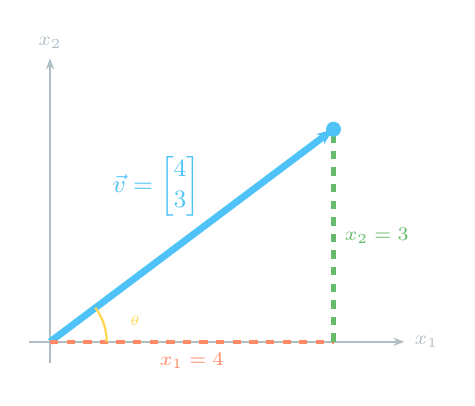
\begin{tikzpicture}[scale=0.9]
          % Axes
          \draw[-{Stealth[length=4pt]}, labelgray, line width=0.8pt] (-0.3,0) -- (5,0) node[right, font=\scriptsize] {$x_1$};
          \draw[-{Stealth[length=4pt]}, labelgray, line width=0.8pt] (0,-0.3) -- (0,4) node[above, font=\scriptsize] {$x_2$};
          % Vector
          \draw[-{Stealth[length=6pt]}, vectora, line width=2.5pt] (0,0) -- (4,3);
          % Components
          \draw[vectorb, line width=1.5pt, dashed] (0,0) -- (4,0) node[midway, below, font=\scriptsize] {\textcolor{vectorb}{$x_1 = 4$}};
          \draw[resultant, line width=1.5pt, dashed] (4,0) -- (4,3) node[midway, right, font=\scriptsize] {\textcolor{resultant}{$x_2 = 3$}};
          % Dot at tip
          \fill[vectora] (4,3) circle (3pt);
          % Label
          \node[vectora, font=\small] at (1.5, 2.2) {$\vec{v} = \begin{bmatrix} 4 \\ 3 \end{bmatrix}$};
          % Angle
          \draw[accent, line width=0.8pt] (0.8,0) arc[start angle=0, end angle=37, radius=0.8];
          \node[accent, font=\tiny] at (1.2, 0.3) {$\theta$};
        \end{tikzpicture}
      \end{center}
    \end{column}
    \begin{column}{0.46\textwidth}
      \textcolor{accent}{\textbf{Components:}}
      {\small
      \begin{itemize}
        \item $\vec{v} = \begin{bmatrix} v_1 \\ v_2 \\ \vdots \\ v_n \end{bmatrix}$ where each $v_i$ is a \textcolor{vectora}{component}
        \item \textcolor{vectorb}{$v_1$} = horizontal extent
        \item \textcolor{resultant}{$v_2$} = vertical extent
      \end{itemize}
      }

      \vspace{0.3cm}
      \textcolor{accent}{\textbf{Dimension:}}
      {\small
      \begin{itemize}
        \item Number of components = \textbf{dimension}
        \item $\vec{v} \in \mathbb{R}^2$ \textemdash\ a \textcolor{vectora}{2D vector}
        \item $\vec{w} \in \mathbb{R}^n$ \textemdash\ an \textcolor{vectora}{$n$-dimensional vector}
      \end{itemize}
      }
    \end{column}
  \end{columns}

  \vspace{0.3cm}
  \begin{center}
    \colorbox{cardbg}{\parbox{0.85\textwidth}{%
      \centering\vspace{3pt}
      {\small\textcolor{accent}{\textbf{Direction:}} $\theta = \arctan\!\left(\frac{v_2}{v_1}\right)$
       \qquad \textcolor{accent}{\textbf{Magnitude:}} $\|\vec{v}\| = \sqrt{v_1^2 + v_2^2}$}
      \vspace{3pt}
    }}
  \end{center}
\end{frame}


% SLIDE 6: Vectors in 3D
\begin{frame}{Vectors in Higher Dimensions}
  \modulemark{2} \hfill \concepttag{From 2D to $n$D}
  \vspace{0.2cm}

  \begin{columns}[T]
    \begin{column}{0.45\textwidth}
      \textcolor{vectora}{\textbf{3D Vector:}}\\[4pt]
      $\vec{v} = \begin{bmatrix} v_1 \\ v_2 \\ v_3 \end{bmatrix} \in \mathbb{R}^3$

      \vspace{0.3cm}
      \begin{center}
        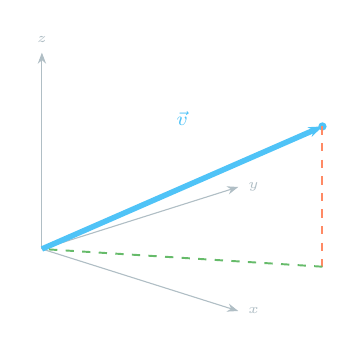
\begin{tikzpicture}[scale=0.75, x={(0.95cm,-0.3cm)}, y={(0.95cm,0.3cm)}, z={(0cm,0.95cm)}]
          % Axes
          \draw[-{Stealth[length=4pt]}, labelgray] (0,0,0) -- (3.5,0,0) node[right, font=\tiny] {$x$};
          \draw[-{Stealth[length=4pt]}, labelgray] (0,0,0) -- (0,3.5,0) node[right, font=\tiny] {$y$};
          \draw[-{Stealth[length=4pt]}, labelgray] (0,0,0) -- (0,0,3.5) node[above, font=\tiny] {$z$};
          % Vector
          \draw[-{Stealth[length=5pt]}, vectora, line width=2pt] (0,0,0) -- (3,2,2.5);
          \fill[vectora] (3,2,2.5) circle (2pt);
          % Projections
          \draw[vectorb, dashed, line width=0.7pt] (3,2,2.5) -- (3,2,0);
          \draw[resultant, dashed, line width=0.7pt] (3,2,0) -- (0,0,0);
          \node[vectora, font=\scriptsize] at (2, 0.5, 2.8) {$\vec{v}$};
        \end{tikzpicture}
      \end{center}
    \end{column}
    \begin{column}{0.50\textwidth}
      \textcolor{accent}{\textbf{Beyond 3D \textemdash\ $n$-dimensional vectors:}}

      \vspace{0.2cm}
      {\small
      \begin{itemize}
        \item We \textbf{cannot visualize} $\mathbb{R}^n$ for $n > 3$
        \item But the \textbf{math works identically}
        \item In data science, $n$ = \textbf{number of features}
      \end{itemize}
      }

      \vspace{0.3cm}
      \colorbox{cardbg}{\parbox{0.9\textwidth}{%
        \vspace{3pt}
        \textcolor{vectorb}{\textbf{\scriptsize Example:}} {\tiny A patient with 5 measurements}\\[2pt]
        {\small $\vec{p} = \begin{bmatrix} 58 \\ 122 \\ 85 \\ 36.7 \\ 98 \end{bmatrix}$
        $\leftarrow$ \scriptsize \textcolor{labelgray}{Age, BP, Weight, Temp, HR}}
        \vspace{3pt}
      }}

      \vspace{0.2cm}
      {\scriptsize\textcolor{labelgray}{Each feature adds a dimension. Real ML models use vectors with \textbf{hundreds or thousands} of dimensions.}}
    \end{column}
  \end{columns}
\end{frame}


% SLIDE 7: Embeddings
\begin{frame}{Vectors as Embeddings}
  \modulemark{2} \hfill \concepttag{Text $\to$ Vector $\to$ Meaning}
  \vspace{0.2cm}

  \begin{center}
    
\begin{tikzpicture}[
      box/.style={draw=vectora, rounded corners=3pt, fill=codebg, minimum width=2cm, minimum height=0.7cm, font=\scriptsize, text=textwhite},
      arrow/.style={-{Stealth[length=4pt]}, vectora, line width=1pt}
    ]
      \node[box] (text) at (0,0) {``King''};
      \node[box, draw=vectorb] (model) at (3.5,0) {Embedding Model};
      \node[box, draw=accent, minimum width=3cm] (vec) at (8,0) {$[0.2,\, -0.5,\, 0.8,\, \ldots]$};
      \draw[arrow] (text) -- (model);
      \draw[arrow, vectorb] (model) -- (vec);
    \end{tikzpicture}
  \end{center}

  \vspace{0.2cm}

  \begin{columns}[T]
    \begin{column}{0.48\textwidth}
      \textcolor{accent}{\textbf{The magic of embeddings:}}\\[4pt]
      {\small
      \begin{itemize}
        \item Words, images, audio $\to$ dense vectors
        \item \textbf{Similar meanings} $\to$ \textbf{nearby vectors}
        \item Arithmetic on meaning!
      \end{itemize}
      }

      \vspace{0.2cm}
      \colorbox{cardbg}{\parbox{0.9\textwidth}{%
        \vspace{3pt}
        \centering
        {\small $\vec{\text{King}} - \vec{\text{Man}} + \vec{\text{Woman}} \approx \vec{\text{Queen}}$}
        \vspace{3pt}
      }}
      {\tiny\textcolor{labelgray}{\hfill --- Roberts, LA for 21st Century}}
    \end{column}
    \begin{column}{0.48\textwidth}
      \textcolor{accent}{\textbf{What gets embedded:}}

      \vspace{0.1cm}
      {\small
      \begin{tabular}{ll}
        \textcolor{vectora}{\textbf{Data}} & \textcolor{vectora}{\textbf{Vector}} \\
        \midrule
        Text / Words & Word2Vec, BERT \\
        Images & CNN features, CLIP \\
        Audio & Mel spectrograms \\
        Graphs & Node2Vec \\
      \end{tabular}
      }

      \vspace{0.2cm}
      {\scriptsize\textcolor{labelgray}{Modern AI = converting everything into vectors, then doing linear algebra on them.}}
    \end{column}
  \end{columns}
\end{frame}


% ============================================================
% MODULE 3: Real-World Vector Examples
% ============================================================

% SLIDE 8: Vectors Everywhere
\begin{frame}{Vectors Are Everywhere}
  \modulemark{3} \hfill \concepttag{Real-World Examples}
  \vspace{0.15cm}

  \begin{columns}[T]
    \begin{column}{0.48\textwidth}
      \minicard{vectora}{Physics: Force}{%
        $\vec{F} = \begin{bmatrix} F_x \\ F_y \end{bmatrix}$
        \quad Magnitude + Direction
      }

      \vspace{0.15cm}
      \minicard{vectorb}{Color: RGB}{%
        $\vec{c} = \begin{bmatrix} 255 \\ 165 \\ 0 \end{bmatrix}$ = Orange
        \quad Each pixel is a 3D vector!
      }

      \vspace{0.15cm}
      \minicard{resultant}{Audio Signal}{%
        $\vec{s} = [s_1, s_2, \ldots, s_{44100}]$
        \quad 1 second at 44.1kHz = 44100-dim vector
      }
    \end{column}
    \begin{column}{0.48\textwidth}
      \minicard{projection}{Portfolio}{%
        $\vec{w} = \begin{bmatrix} 100 \\ -50 \\ 200 \end{bmatrix}$ = Holdings
        \quad Long/short positions in 3 stocks
      }

      \vspace{0.15cm}
      \minicard{accent}{Word Count (BoW)}{%
        ``data science is fun'' $\to$
        $[2,\, 2,\, 1,\, 1]$ counts per word
      }

      \vspace{0.15cm}
      \minicard{vectora}{Customer Purchase}{%
        $\vec{p} = \begin{bmatrix} 100 \\ 50 \\ 75 \end{bmatrix}$
        \quad Spend per category
      }
    \end{column}
  \end{columns}

  \vspace{0.25cm}
  \begin{center}
    \colorbox{cardbg}{\parbox{0.85\textwidth}{%
      \centering\vspace{3pt}
      {\small\textcolor{accent}{\textbf{Pattern:}} \textcolor{textwhite}{Any structured collection of measurements can be represented as a vector. The dimension equals the number of measurements.}}
      \vspace{3pt}
    }}
  \end{center}
\end{frame}


% ============================================================
% MODULE 4: Types of Vectors
% ============================================================

% SLIDE 9: Types of Vectors
\begin{frame}{Types of Vectors}
  \modulemark{4} \hfill \concepttag{Classification}
  \vspace{0.2cm}

  \begin{columns}[T]
    \begin{column}{0.48\textwidth}
      \textcolor{vectora}{\textbf{Row vs Column Vector:}}\\[4pt]
      {\small
        Row: $\vec{v}^T = \begin{bmatrix} 1 & 2 & 3 \end{bmatrix}$ {\tiny (1$\times$n)}\\[6pt]
        Column: $\vec{v} = \begin{bmatrix} 1 \\ 2 \\ 3 \end{bmatrix}$ {\tiny (n$\times$1)}
      }

      \vspace{0.3cm}
      \textcolor{vectorb}{\textbf{Zero Vector:}}\\[4pt]
      {\small $\vec{0} = \begin{bmatrix} 0 \\ 0 \\ 0 \\ 0 \end{bmatrix}$ \quad No magnitude, no direction}

      \vspace{0.3cm}
      \textcolor{resultant}{\textbf{Ones Vector:}}\\[4pt]
      {\small $\mathbf{1} = \begin{bmatrix} 1 \\ 1 \\ 1 \\ 1 \end{bmatrix}$ \quad Used for averaging: $\bar{x} = \frac{1}{n}\mathbf{1}^T\vec{x}$}
    \end{column}
    \begin{column}{0.48\textwidth}
      \textcolor{accent}{\textbf{Unit Vector:}}\\[4pt]
      {\small $\|\hat{v}\| = 1$ \quad Direction without magnitude}\\[4pt]
      {\small Standard basis: $\hat{\imath} = \begin{bmatrix} 1 \\ 0 \end{bmatrix}$, $\hat{\jmath} = \begin{bmatrix} 0 \\ 1 \end{bmatrix}$}

      \vspace{0.3cm}
      \textcolor{projection}{\textbf{Standard Basis Vectors:}}\\[4pt]
      {\small $\vec{e}_i$ has 1 in position $i$, 0 elsewhere}\\[4pt]
      {\small $\vec{e}_3 = \begin{bmatrix} 0 \\ 0 \\ 1 \\ 0 \end{bmatrix} \in \mathbb{R}^4$}

      \vspace{0.3cm}
      \textcolor{vectora}{\textbf{Equal Vectors:}}\\[4pt]
      {\small $\vec{a} = \vec{b}$ iff $a_i = b_i$ for all $i$}\\[2pt]
      {\scriptsize Same magnitude \textbf{and} same direction}
    \end{column}
  \end{columns}
\end{frame}


% SLIDE 10: Python Representations
\begin{frame}{Vectors in Python}
  \modulemark{4} \hfill \concepttag{Code}
  \vspace{0.2cm}

  \begin{columns}[T]
    \begin{column}{0.48\textwidth}
      \colorbox{codebg}{\parbox{0.92\textwidth}{%
        \vspace{4pt}
        {\ttfamily\scriptsize
        \textcolor{resultant}{import} \textcolor{textwhite}{numpy} \textcolor{resultant}{as} \textcolor{textwhite}{np}\\[4pt]
        \textcolor{labelgray}{\# Column vector}\\
        \textcolor{textwhite}{v = np.array([}\textcolor{accent}{58}\textcolor{textwhite}{,} \textcolor{accent}{122}\textcolor{textwhite}{])}\\[4pt]
        \textcolor{labelgray}{\# Zero vector}\\
        \textcolor{textwhite}{z = np.zeros(}\textcolor{accent}{4}\textcolor{textwhite}{)}\\[4pt]
        \textcolor{labelgray}{\# Ones vector}\\
        \textcolor{textwhite}{o = np.ones(}\textcolor{accent}{4}\textcolor{textwhite}{)}\\[4pt]
        \textcolor{labelgray}{\# Unit vector (normalize)}\\
        \textcolor{textwhite}{u = v / np.linalg.norm(v)}\\[4pt]
        \textcolor{labelgray}{\# Standard basis}\\
        \textcolor{textwhite}{e2 = np.eye(}\textcolor{accent}{4}\textcolor{textwhite}{)[}\textcolor{accent}{1}\textcolor{textwhite}{]}
        }
        \vspace{4pt}
      }}
    \end{column}
    \begin{column}{0.48\textwidth}
      \textcolor{accent}{\textbf{Key NumPy facts:}}

      \vspace{0.15cm}
      {\small
      \begin{itemize}
        \item \texttt{np.array} creates vectors
        \item \texttt{np.zeros(n)} $\to$ zero vector
        \item \texttt{np.ones(n)} $\to$ ones vector
        \item \texttt{np.eye(n)[i]} $\to$ $\vec{e}_i$
        \item \texttt{v / np.linalg.norm(v)} $\to$ unit vector
        \item \texttt{v.shape} $\to$ dimension
      \end{itemize}
      }

      \vspace{0.2cm}
      \colorbox{cardbg}{\parbox{0.9\textwidth}{%
        \vspace{3pt}
        {\scriptsize\textcolor{accent}{\textbf{Tip:}} NumPy 1D arrays are \textit{neither} row nor column --- they are just arrays. Use \texttt{v.reshape(-1,1)} for explicit column.}
        \vspace{3pt}
      }}
    \end{column}
  \end{columns}
\end{frame}


% ============================================================
% MODULE 5: Vector Operations
% ============================================================

% SLIDE 11: Vector Addition & Subtraction
\begin{frame}{Vector Addition \& Subtraction}
  \modulemark{5} \hfill \concepttag{Operations}
  \vspace{0.15cm}

  \begin{columns}[T]
    \begin{column}{0.48\textwidth}
      \textcolor{vectora}{\textbf{Addition:}}\\[4pt]
      {\small $\vec{a} + \vec{b} = \begin{bmatrix} a_1 + b_1 \\ a_2 + b_2 \end{bmatrix}$}

      \vspace{0.15cm}
      \begin{center}
      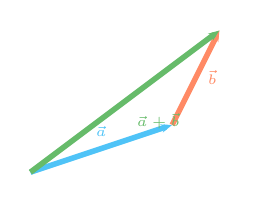
\begin{tikzpicture}[scale=0.6]
        \draw[-{Stealth[length=4pt]}, vectora, line width=2pt] (0,0) -- (3,1) node[midway, above, font=\tiny] {$\vec{a}$};
        \draw[-{Stealth[length=4pt]}, vectorb, line width=2pt] (3,1) -- (4,3) node[midway, right, font=\tiny] {$\vec{b}$};
        \draw[-{Stealth[length=4pt]}, resultant, line width=2pt] (0,0) -- (4,3) node[midway, below right, font=\tiny] {$\vec{a}+\vec{b}$};
      \end{tikzpicture}
      \end{center}

      {\scriptsize\textcolor{labelgray}{Triangle law: place $\vec{b}$ at tip of $\vec{a}$}}

      \vspace{0.15cm}
      \textcolor{accent}{\textbf{Example:}}\\
      {\small $\begin{bmatrix} 1 \\ 3 \end{bmatrix} + \begin{bmatrix} 4 \\ 2 \end{bmatrix} = \begin{bmatrix} 5 \\ 5 \end{bmatrix}$}
    \end{column}
    \begin{column}{0.48\textwidth}
      \textcolor{vectorb}{\textbf{Subtraction:}}\\[4pt]
      {\small $\vec{a} - \vec{b} = \begin{bmatrix} a_1 - b_1 \\ a_2 - b_2 \end{bmatrix}$}

      \vspace{0.15cm}
      \begin{center}
      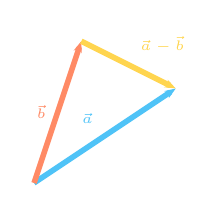
\begin{tikzpicture}[scale=0.6]
        \draw[-{Stealth[length=4pt]}, vectora, line width=2pt] (0,0) -- (3,2) node[midway, above left, font=\tiny] {$\vec{a}$};
        \draw[-{Stealth[length=4pt]}, vectorb, line width=2pt] (0,0) -- (1,3) node[midway, left, font=\tiny] {$\vec{b}$};
        \draw[-{Stealth[length=4pt]}, accent, line width=2pt] (1,3) -- (3,2) node[midway, above right, font=\tiny] {$\vec{a}-\vec{b}$};
      \end{tikzpicture}
      \end{center}

      {\scriptsize\textcolor{labelgray}{$\vec{a} - \vec{b}$ points from tip of $\vec{b}$ to tip of $\vec{a}$}}

      \vspace{0.15cm}
      \textcolor{accent}{\textbf{Properties:}}\\
      {\scriptsize
        Commutative: $\vec{a} + \vec{b} = \vec{b} + \vec{a}$\\
        Associative: $(\vec{a} + \vec{b}) + \vec{c} = \vec{a} + (\vec{b} + \vec{c})$\\
        Identity: $\vec{a} + \vec{0} = \vec{a}$\\
        Inverse: $\vec{a} + (-\vec{a}) = \vec{0}$
      }
    \end{column}
  \end{columns}
\end{frame}


% SLIDE 12: Scalar Multiplication
\begin{frame}{Scalar Multiplication}
  \modulemark{5} \hfill \concepttag{Scaling Vectors}
  \vspace{0.2cm}

  \begin{columns}[T]
    \begin{column}{0.45\textwidth}
      \textcolor{accent}{\textbf{Definition:}}\\[4pt]
      {\small $k\vec{v} = \begin{bmatrix} kv_1 \\ kv_2 \\ \vdots \\ kv_n \end{bmatrix}$}

      \vspace{0.3cm}
      \begin{center}
      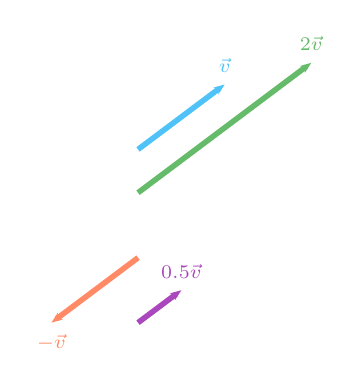
\begin{tikzpicture}[scale=0.55]
        \draw[-{Stealth[length=4pt]}, vectora, line width=2pt] (0,0) -- (2,1.5) node[above, font=\scriptsize] {$\vec{v}$};
        \draw[-{Stealth[length=4pt]}, resultant, line width=2pt] (0,-1) -- (4,-1+3) node[above, font=\scriptsize] {$2\vec{v}$};
        \draw[-{Stealth[length=4pt]}, vectorb, line width=2pt] (0,-2.5) -- (-2,-2.5-1.5) node[below, font=\scriptsize] {$-\vec{v}$};
        \draw[-{Stealth[length=4pt]}, projection, line width=2pt] (0,-4) -- (1,-4+0.75) node[above, font=\scriptsize] {$0.5\vec{v}$};
      \end{tikzpicture}
      \end{center}
    \end{column}
    \begin{column}{0.50\textwidth}
      \textcolor{accent}{\textbf{What happens:}}\\[6pt]
      {\small
      \begin{tabular}{ll}
        $k > 1$ & \textcolor{resultant}{Stretches} (same direction) \\[2pt]
        $0 < k < 1$ & \textcolor{projection}{Shrinks} (same direction) \\[2pt]
        $k = 0$ & Zero vector $\vec{0}$ \\[2pt]
        $k < 0$ & \textcolor{vectorb}{Reverses} direction \\[2pt]
        $k = -1$ & \textcolor{vectorb}{Flips} (additive inverse) \\
      \end{tabular}
      }

      \vspace{0.3cm}
      \textcolor{accent}{\textbf{Example:}}\\[4pt]
      {\small $3 \cdot \begin{bmatrix} 2 \\ -1 \end{bmatrix} = \begin{bmatrix} 6 \\ -3 \end{bmatrix}$}

      \vspace{0.2cm}
      {\scriptsize
        Distributive: $k(\vec{a} + \vec{b}) = k\vec{a} + k\vec{b}$\\
        $(k + l)\vec{a} = k\vec{a} + l\vec{a}$
      }
    \end{column}
  \end{columns}
\end{frame}


% ============================================================
% MODULE 6: Norms
% ============================================================

% SLIDE 13: Norms — Measuring Vectors
\begin{frame}{Norms \textemdash\ Measuring Vector Length}
  \modulemark{6} \hfill \concepttag{L1, L2, L$\infty$}
  \vspace{0.15cm}

  \begin{columns}[T]
    \begin{column}{0.50\textwidth}
      \textcolor{vectora}{\textbf{Euclidean Norm (L$_2$):}}\\[4pt]
      {\small $\|\vec{v}\|_2 = \sqrt{\sum_{i=1}^n v_i^2}$}\\[6pt]
      {\scriptsize Straight-line distance. Most common in ML.}

      \vspace{0.3cm}
      \textcolor{vectorb}{\textbf{Manhattan Norm (L$_1$):}}\\[4pt]
      {\small $\|\vec{v}\|_1 = \sum_{i=1}^n |v_i|$}\\[6pt]
      {\scriptsize City-block distance. Robust to outliers.}

      \vspace{0.3cm}
      \textcolor{projection}{\textbf{Chebyshev Norm (L$_\infty$):}}\\[4pt]
      {\small $\|\vec{v}\|_\infty = \max_i |v_i|$}\\[6pt]
      {\scriptsize Maximum absolute component.}
    \end{column}
    \begin{column}{0.46\textwidth}
      \textcolor{accent}{\textbf{Example:}} $\vec{v} = \begin{bmatrix} 3 \\ -4 \end{bmatrix}$

      \vspace{0.2cm}
      {\small
      \begin{tabular}{ll}
        \textcolor{vectora}{$\|\vec{v}\|_2$} & $= \sqrt{9 + 16} = \textcolor{vectora}{5}$ \\[4pt]
        \textcolor{vectorb}{$\|\vec{v}\|_1$} & $= |3| + |-4| = \textcolor{vectorb}{7}$ \\[4pt]
        \textcolor{projection}{$\|\vec{v}\|_\infty$} & $= \max(3, 4) = \textcolor{projection}{4}$ \\
      \end{tabular}
      }

      \vspace{0.3cm}
      \textcolor{accent}{\textbf{Properties of norms:}}\\[4pt]
      {\scriptsize
      \begin{itemize}
        \item $\|\vec{v}\| \geq 0$ \quad (non-negative)
        \item $\|\vec{v}\| = 0 \iff \vec{v} = \vec{0}$
        \item $\|k\vec{v}\| = |k|\,\|\vec{v}\|$ \quad (scaling)
        \item $\|\vec{a} + \vec{b}\| \leq \|\vec{a}\| + \|\vec{b}\|$ \quad (triangle ineq.)
      \end{itemize}
      }
    \end{column}
  \end{columns}
\end{frame}


% SLIDE 14: Unit Balls & Norm Geometry
\begin{frame}{Geometry of Norms \textemdash\ Unit Balls}
  \modulemark{6} \hfill \concepttag{Visualization}
  \vspace{0.2cm}

  \begin{center}
    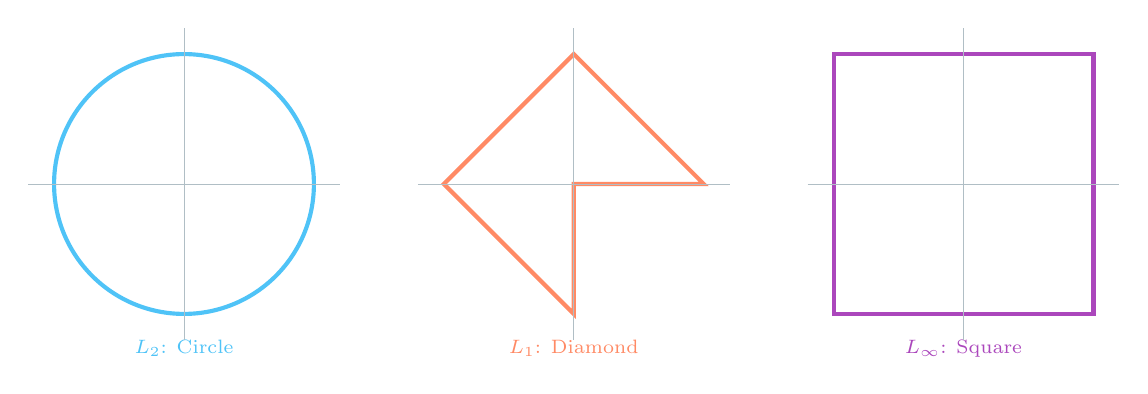
\begin{tikzpicture}[scale=1.1]
      % L2 - circle
      \draw[vectora, line width=1.5pt] (0,0) circle (1.5);
      \node[vectora, font=\scriptsize] at (0, -1.9) {$L_2$: Circle};

      % L1 - diamond
      \draw[vectorb, line width=1.5pt] (4.5,0) -- (4.5+1.5,0+0) -- (4.5,1.5) -- (4.5-1.5,0) -- (4.5,-1.5) -- cycle;
      \node[vectorb, font=\scriptsize] at (4.5, -1.9) {$L_1$: Diamond};

      % Linf - square
      \draw[projection, line width=1.5pt] (9-1.5,-1.5) rectangle (9+1.5,1.5);
      \node[projection, font=\scriptsize] at (9, -1.9) {$L_\infty$: Square};

      % Axes for each
      \foreach \cx in {0, 4.5, 9} {
        \draw[labelgray, line width=0.3pt] (\cx-1.8,0) -- (\cx+1.8,0);
        \draw[labelgray, line width=0.3pt] (\cx,-1.8) -- (\cx,1.8);
      }
    \end{tikzpicture}
  \end{center}

  \vspace{0.2cm}
  \begin{center}
    \colorbox{cardbg}{\parbox{0.88\textwidth}{%
      \centering\vspace{4pt}
      {\small\textcolor{accent}{\textbf{Unit ball}} = set of all vectors with $\|\vec{v}\| \leq 1$.
       The \textbf{shape} reveals how each norm ``measures'' distance.
       $L_1$ penalizes sparse solutions less $\Rightarrow$ used in \textbf{Lasso regularization}.}
      \vspace{4pt}
    }}
  \end{center}
\end{frame}


% SLIDE 15: Distance Between Vectors
\begin{frame}{Distance Between Vectors}
  \modulemark{6} \hfill \concepttag{Measuring Similarity}
  \vspace{0.2cm}

  \begin{columns}[T]
    \begin{column}{0.48\textwidth}
      \textcolor{accent}{\textbf{Definition:}}\\[4pt]
      {\small $d(\vec{a}, \vec{b}) = \|\vec{a} - \vec{b}\|$}

      \vspace{0.2cm}
      \textcolor{vectora}{\textbf{Euclidean distance:}}\\[4pt]
      {\small $d_2(\vec{a}, \vec{b}) = \sqrt{\sum_{i=1}^n (a_i - b_i)^2}$}

      \vspace{0.2cm}
      \textcolor{accent}{\textbf{Example:}}\\[4pt]
      {\small $\vec{a} = \begin{bmatrix} 1 \\ 3 \end{bmatrix}$, $\vec{b} = \begin{bmatrix} 4 \\ 7 \end{bmatrix}$}\\[6pt]
      {\small $d = \sqrt{(4-1)^2 + (7-3)^2} = \sqrt{9+16} = 5$}
    \end{column}
    \begin{column}{0.48\textwidth}
      \begin{center}
      \begin{tikzpicture}[scale=0.55]
        \draw[-{Stealth[length=3pt]}, labelgray, line width=0.5pt] (-0.5,0) -- (6,0);
        \draw[-{Stealth[length=3pt]}, labelgray, line width=0.5pt] (0,-0.5) -- (0,5.5);
        % Points
        \fill[vectora] (1,3) circle (4pt);
        \node[vectora, font=\scriptsize, above left] at (1,3) {$\vec{a}$};
        \fill[vectorb] (4,4.5) circle (4pt);
        \node[vectorb, font=\scriptsize, above right] at (4,4.5) {$\vec{b}$};
        % Distance line
        \draw[accent, line width=1.5pt, dashed] (1,3) -- (4,4.5);
        \node[accent, font=\scriptsize, below right] at (2.5,3.5) {$d=5$};
      \end{tikzpicture}
      \end{center}

      \vspace{0.1cm}
      \textcolor{accent}{\textbf{Python:}}\\[2pt]
      \colorbox{codebg}{\parbox{0.85\textwidth}{%
        \vspace{2pt}
        {\ttfamily\tiny
        d = np.linalg.norm(a - b)
        }
        \vspace{2pt}
      }}

      \vspace{0.15cm}
      {\scriptsize\textcolor{labelgray}{Small distance = similar data points.\\This is the foundation of KNN, clustering, recommendation systems.}}
    \end{column}
  \end{columns}
\end{frame}


% ============================================================
% MODULE 7: Nearest Neighbours
% ============================================================

% SLIDE 16: Nearest Neighbour
\begin{frame}{Nearest Neighbour Search}
  \modulemark{7} \hfill \concepttag{Finding Similar Data}
  \vspace{0.2cm}

  \begin{columns}[T]
    \begin{column}{0.48\textwidth}
      \textcolor{accent}{\textbf{Problem:}} Given a query point $\vec{q}$, find the closest point in a dataset.

      \vspace{0.2cm}
      {\small $\text{NN}(\vec{q}) = \arg\min_{\vec{x}_i} \|\vec{q} - \vec{x}_i\|$}

      \vspace{0.2cm}
      \begin{center}
      \begin{tikzpicture}[scale=0.55]
        \draw[-{Stealth[length=3pt]}, labelgray, line width=0.5pt] (-0.5,0) -- (6,0);
        \draw[-{Stealth[length=3pt]}, labelgray, line width=0.5pt] (0,-0.5) -- (0,5.5);
        % Data points
        \fill[vectora] (1,2) circle (3pt);
        \fill[vectora] (2,4) circle (3pt);
        \fill[vectora] (3,1) circle (3pt);
        \fill[vectora] (4.5,3.5) circle (3pt);
        \fill[vectora] (5,1.5) circle (3pt);
        % Query
        \fill[accent] (3.5,3) circle (4pt);
        \node[accent, font=\scriptsize, right] at (3.6,3) {$\vec{q}$};
        % Nearest
        \draw[accent, dashed, line width=1pt] (3.5,3) -- (4.5,3.5);
        \draw[resultant, line width=1.5pt] (4.5,3.5) circle (5pt);
        \node[resultant, font=\tiny, right] at (4.8,3.5) {NN};
      \end{tikzpicture}
      \end{center}
    \end{column}
    \begin{column}{0.48\textwidth}
      \textcolor{accent}{\textbf{Distance Matrix:}}\\[4pt]
      {\scriptsize All pairwise distances:}

      \vspace{0.1cm}
      {\small $D_{ij} = \|\vec{x}_i - \vec{x}_j\|$}

      \vspace{0.2cm}
      \colorbox{codebg}{\parbox{0.9\textwidth}{%
        \vspace{3pt}
        {\ttfamily\tiny
        \textcolor{resultant}{import} numpy \textcolor{resultant}{as} np\\[2pt]
        X = np.array([[58,122],[71,110],\\
        \hspace{2.2cm}[48,110],[34,123]])\\[2pt]
        q = np.array([50, 115])\\[2pt]
        \textcolor{labelgray}{\# Distances to all points}\\
        dists = [np.linalg.norm(q - x)\\
        \hspace{1.5cm}\textcolor{resultant}{for} x \textcolor{resultant}{in} X]\\[2pt]
        nn = np.argmin(dists)\\
        \textcolor{resultant}{print}(f"Nearest: \{nn\}")
        }
        \vspace{3pt}
      }}

      \vspace{0.15cm}
      {\scriptsize\textcolor{labelgray}{Used in: KNN classification, recommendation engines, image search, anomaly detection.}}
    \end{column}
  \end{columns}
\end{frame}


% ============================================================
% MODULE 8: Dot Product / Inner Product
% ============================================================

% SLIDE 17: Dot Product Definition
\begin{frame}{The Dot Product}
  \modulemark{8} \hfill \concepttag{Inner Product}
  \vspace{0.2cm}

  \begin{columns}[T]
    \begin{column}{0.48\textwidth}
      \textcolor{accent}{\textbf{Algebraic definition:}}\\[6pt]
      {\small $\vec{a} \cdot \vec{b} = \sum_{i=1}^n a_i b_i = a_1 b_1 + a_2 b_2 + \cdots + a_n b_n$}

      \vspace{0.3cm}
      \textcolor{vectora}{\textbf{Geometric definition:}}\\[6pt]
      {\small $\vec{a} \cdot \vec{b} = \|\vec{a}\|\, \|\vec{b}\|\, \cos\theta$}

      \vspace{0.3cm}
      \textcolor{accent}{\textbf{Example:}}\\[4pt]
      {\small $\begin{bmatrix} 1 \\ 2 \\ 3 \end{bmatrix} \cdot \begin{bmatrix} 4 \\ -5 \\ 6 \end{bmatrix} = 4 + (-10) + 18 = 12$}

      \vspace{0.2cm}
      \colorbox{codebg}{\parbox{0.85\textwidth}{%
        \vspace{2pt}
        {\ttfamily\tiny np.dot(a, b) \textcolor{labelgray}{\# or a @ b}}
        \vspace{2pt}
      }}
    \end{column}
    \begin{column}{0.48\textwidth}
      \textcolor{accent}{\textbf{What the sign tells you:}}

      \vspace{0.15cm}
      \begin{center}
      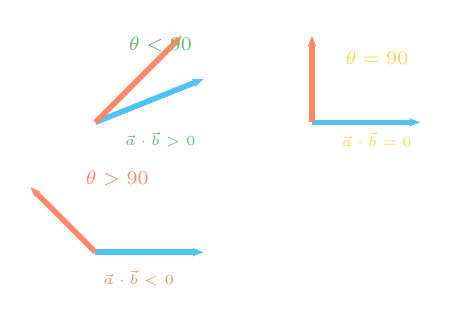
\begin{tikzpicture}[scale=0.55]
        % Positive
        \draw[-{Stealth[length=4pt]}, vectora, line width=2pt] (0,0) -- (2.5,1);
        \draw[-{Stealth[length=4pt]}, vectorb, line width=2pt] (0,0) -- (2,2);
        \node[resultant, font=\scriptsize] at (1.5, 1.8) {$\theta < 90°$};
        \node[resultant, font=\tiny] at (1.5, -0.4) {$\vec{a}\cdot\vec{b} > 0$};

        % Zero
        \draw[-{Stealth[length=4pt]}, vectora, line width=2pt] (5,0) -- (7.5,0);
        \draw[-{Stealth[length=4pt]}, vectorb, line width=2pt] (5,0) -- (5,2);
        \node[accent, font=\scriptsize] at (6.5, 1.5) {$\theta = 90°$};
        \node[accent, font=\tiny] at (6.5, -0.4) {$\vec{a}\cdot\vec{b} = 0$};

        % Negative
        \draw[-{Stealth[length=4pt]}, vectora, line width=2pt] (0,-3) -- (2.5,-3);
        \draw[-{Stealth[length=4pt]}, vectorb, line width=2pt] (0,-3) -- (-1.5,-1.5);
        \node[vectorb, font=\scriptsize] at (0.5, -1.3) {$\theta > 90°$};
        \node[vectorb, font=\tiny] at (1, -3.6) {$\vec{a}\cdot\vec{b} < 0$};
      \end{tikzpicture}
      \end{center}

      \vspace{0.1cm}
      \textcolor{accent}{\textbf{Properties:}}\\
      {\scriptsize
        Commutative: $\vec{a}\cdot\vec{b} = \vec{b}\cdot\vec{a}$\\
        Distributive: $\vec{a}\cdot(\vec{b}+\vec{c}) = \vec{a}\cdot\vec{b} + \vec{a}\cdot\vec{c}$\\
        Self-dot: $\vec{a}\cdot\vec{a} = \|\vec{a}\|^2$
      }
    \end{column}
  \end{columns}
\end{frame}


% SLIDE 18: Dot Product Applications
\begin{frame}{Dot Product Applications}
  \modulemark{8} \hfill \concepttag{ML, Finance, NLP}
  \vspace{0.15cm}

  \begin{columns}[T]
    \begin{column}{0.48\textwidth}
      \excard{vectora}{ML: Weighted Score}{%
        Features $\vec{x}$, weights $\vec{w}$:\\
        $\text{score} = \vec{w} \cdot \vec{x} = \sum w_i x_i$\\[2pt]
        This is a linear model's prediction!
      }

      \vspace{0.15cm}
      \excard{vectorb}{Finance: NPV}{%
        Cash flows $\vec{c} = [c_0, c_1, \ldots, c_T]$\\
        Discount $\vec{d} = [1, \frac{1}{1+r}, \ldots, \frac{1}{(1+r)^T}]$\\[2pt]
        $\text{NPV} = \vec{c} \cdot \vec{d}$
      }
    \end{column}
    \begin{column}{0.48\textwidth}
      \excard{resultant}{Cosine Similarity}{%
        $\cos\theta = \frac{\vec{a} \cdot \vec{b}}{\|\vec{a}\|\,\|\vec{b}\|}$\\[4pt]
        $\cos\theta = 1$: identical direction\\
        $\cos\theta = 0$: orthogonal\\
        $\cos\theta = -1$: opposite
      }

      \vspace{0.15cm}
      \excard{projection}{De-meaning}{%
        $\tilde{\vec{x}} = \vec{x} - \bar{x}\,\mathbf{1}$\\[2pt]
        Subtract mean from each component.\\
        $\mathbf{1}^T\tilde{\vec{x}} = 0$ (zero sum)
      }
    \end{column}
  \end{columns}

  \vspace{0.1cm}
  \begin{center}
    {\scriptsize\textcolor{labelgray}{The dot product is the most important single operation in all of machine learning.}}
  \end{center}
\end{frame}


% ============================================================
% MODULE 9: Projection
% ============================================================

% SLIDE 19: Projection of Vectors
\begin{frame}{Projection of Vectors}
  \modulemark{9} \hfill \concepttag{Orthogonal Projection}
  \vspace{0.15cm}

  \begin{columns}[T]
    \begin{column}{0.48\textwidth}
      \textcolor{accent}{\textbf{Scalar projection:}}\\[4pt]
      {\small $\text{comp}_{\vec{v}}\vec{u} = \frac{\vec{u} \cdot \vec{v}}{\|\vec{v}\|}$}

      \vspace{0.3cm}
      \textcolor{vectora}{\textbf{Vector projection:}}\\[4pt]
      {\small $\text{proj}_{\vec{v}}\vec{u} = \frac{\vec{u} \cdot \vec{v}}{\|\vec{v}\|^2}\,\vec{v}$}

      \vspace{0.3cm}
      \begin{center}
      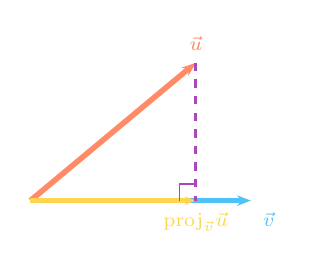
\begin{tikzpicture}[scale=0.7]
        \draw[-{Stealth[length=5pt]}, vectora, line width=2pt] (0,0) -- (4,0) node[below right, font=\scriptsize] {$\vec{v}$};
        \draw[-{Stealth[length=5pt]}, vectorb, line width=2pt] (0,0) -- (3,2.5) node[above, font=\scriptsize] {$\vec{u}$};
        % Projection
        \draw[-{Stealth[length=4pt]}, accent, line width=2pt] (0,0) -- (3,0) node[below, font=\scriptsize] {$\text{proj}_{\vec{v}}\vec{u}$};
        % Perpendicular
        \draw[projection, dashed, line width=1pt] (3,2.5) -- (3,0);
        % Right angle
        \draw[projection, line width=0.5pt] (2.7,0) -- (2.7,0.3) -- (3,0.3);
      \end{tikzpicture}
      \end{center}
    \end{column}
    \begin{column}{0.48\textwidth}
      \textcolor{accent}{\textbf{Example:}}\\[4pt]
      {\small $\vec{u} = \begin{bmatrix} 3 \\ 4 \end{bmatrix}$, $\vec{v} = \begin{bmatrix} 4 \\ 3 \end{bmatrix}$}

      \vspace{0.15cm}
      {\small
      $\vec{u} \cdot \vec{v} = 12 + 12 = 24$\\[4pt]
      $\|\vec{v}\|^2 = 16 + 9 = 25$\\[4pt]
      $\text{proj}_{\vec{v}}\vec{u} = \frac{24}{25}\begin{bmatrix} 4 \\ 3 \end{bmatrix} = \begin{bmatrix} 3.84 \\ 2.88 \end{bmatrix}$
      }

      \vspace{0.2cm}
      \colorbox{codebg}{\parbox{0.9\textwidth}{%
        \vspace{2pt}
        {\ttfamily\tiny
        proj = (np.dot(u,v)/np.dot(v,v))*v
        }
        \vspace{2pt}
      }}

      \vspace{0.15cm}
      {\scriptsize\textcolor{labelgray}{Projection decomposes $\vec{u}$ into a component along $\vec{v}$ and a perpendicular residual. This is the geometric heart of \textbf{linear regression} and \textbf{PCA}.}}
    \end{column}
  \end{columns}
\end{frame}


% ============================================================
% MODULE 10: Linear Combinations
% ============================================================

% SLIDE 20: Linear Combinations
\begin{frame}{Linear Combinations}
  \modulemark{10} \hfill \concepttag{Building Blocks of LA}
  \vspace{0.15cm}

  \begin{columns}[T]
    \begin{column}{0.48\textwidth}
      \textcolor{accent}{\textbf{Definition:}}\\[6pt]
      {\small $\vec{v} = c_1\vec{v}_1 + c_2\vec{v}_2 + \cdots + c_k\vec{v}_k$}\\[4pt]
      {\scriptsize where $c_i$ are scalars (coefficients/weights)}

      \vspace{0.3cm}
      \textcolor{vectora}{\textbf{Example:}}\\[4pt]
      {\small
      $2\begin{bmatrix} 1 \\ 0 \end{bmatrix} + 3\begin{bmatrix} 0 \\ 1 \end{bmatrix} = \begin{bmatrix} 2 \\ 3 \end{bmatrix}$
      }

      \vspace{0.15cm}
      \begin{center}
      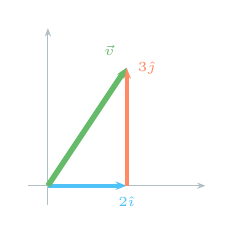
\begin{tikzpicture}[scale=0.5]
        \draw[-{Stealth[length=3pt]}, labelgray, line width=0.4pt] (-0.5,0) -- (4,0);
        \draw[-{Stealth[length=3pt]}, labelgray, line width=0.4pt] (0,-0.5) -- (0,4);
        \draw[-{Stealth[length=4pt]}, vectora, line width=1.5pt] (0,0) -- (2,0) node[below, font=\tiny] {$2\hat\imath$};
        \draw[-{Stealth[length=4pt]}, vectorb, line width=1.5pt] (2,0) -- (2,3) node[right, font=\tiny] {$3\hat\jmath$};
        \draw[-{Stealth[length=4pt]}, resultant, line width=2pt] (0,0) -- (2,3) node[above left, font=\tiny] {$\vec{v}$};
      \end{tikzpicture}
      \end{center}
    \end{column}
    \begin{column}{0.48\textwidth}
      \textcolor{accent}{\textbf{Why it matters:}}

      \vspace{0.15cm}
      {\small
      \begin{itemize}
        \item \textcolor{vectora}{\textbf{Span:}} All possible linear combinations of a set of vectors
        \item \textcolor{vectorb}{\textbf{Basis:}} Minimal spanning set
        \item \textcolor{resultant}{\textbf{Linear independence:}} No vector is a linear combination of the others
      \end{itemize}
      }

      \vspace{0.2cm}
      \textcolor{accent}{\textbf{Applications:}}
      {\scriptsize
      \begin{itemize}
        \item \textbf{Feature engineering}: new features as weighted sums
        \item \textbf{PCA}: data as combination of principal components
        \item \textbf{Linear regression}: $\hat{y} = X\vec{w}$ (prediction as lin.\ combo of features)
        \item \textbf{Neural networks}: each layer computes linear combinations
      \end{itemize}
      }
    \end{column}
  \end{columns}
\end{frame}


% SLIDE 21: Summary & Big Picture
\begin{frame}{The Vector Toolkit \textemdash\ Summary}
  \modulemark{$\Sigma$} \hfill \concepttag{Everything Connects}
  \vspace{0.2cm}

  \begin{center}
    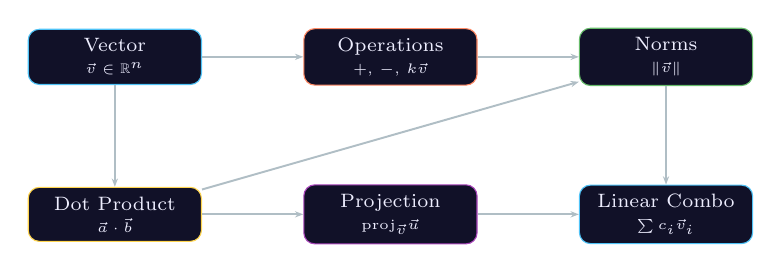
\begin{tikzpicture}[
      concept/.style={draw=vectora, rounded corners=4pt, fill=codebg, minimum width=2.2cm, minimum height=0.65cm, font=\scriptsize, text=textwhite, align=center},
      link/.style={-{Stealth[length=3pt]}, labelgray, line width=0.7pt}
    ]
      % Top row
      \node[concept] (vec) at (0, 2.5) {Vector\\{\tiny $\vec{v} \in \mathbb{R}^n$}};
      \node[concept, draw=vectorb] (ops) at (3.5, 2.5) {Operations\\{\tiny $+$, $-$, $k\vec{v}$}};
      \node[concept, draw=resultant] (norm) at (7, 2.5) {Norms\\{\tiny $\|\vec{v}\|$}};

      % Bottom row
      \node[concept, draw=accent] (dot) at (0, 0.5) {Dot Product\\{\tiny $\vec{a}\cdot\vec{b}$}};
      \node[concept, draw=projection] (proj) at (3.5, 0.5) {Projection\\{\tiny $\text{proj}_{\vec{v}}\vec{u}$}};
      \node[concept, draw=vectora] (lc) at (7, 0.5) {Linear Combo\\{\tiny $\sum c_i\vec{v}_i$}};

      % Links
      \draw[link] (vec) -- (ops);
      \draw[link] (ops) -- (norm);
      \draw[link] (vec) -- (dot);
      \draw[link] (dot) -- (proj);
      \draw[link] (dot) -- (norm);
      \draw[link] (proj) -- (lc);
      \draw[link] (norm) -- (lc);
    \end{tikzpicture}
  \end{center}

  \vspace{0.2cm}
  \begin{center}
    \colorbox{cardbg}{\parbox{0.88\textwidth}{%
      \centering\vspace{4pt}
      {\small\textcolor{accent}{\textbf{The Big Picture:}}
       \textcolor{textwhite}{Vectors are the \textbf{universal language} of data.
       Every ML model, every neural network, every recommendation engine
       operates on vectors. Master these fundamentals, and the rest of
       linear algebra \textemdash\ matrices, transformations, eigenvalues \textemdash\
       becomes a natural extension.}}
      \vspace{4pt}
    }}
  \end{center}

  \vspace{0.15cm}
  \begin{center}
    {\small\textcolor{vectora}{\textbf{Next:}} Matrices, Linear Transformations, Eigenvalues \& SVD}
  \end{center}
\end{frame}


\end{document}
